\appendix
\section{BVH Data Processing Pipeline}
\label{appendix:BVHData}

\subsection{Skeleton Structure of a Character}
\label{appendix:BVHSkeleton}

Some skeleton joint names from the $75$ motion skeletons include:

{
	\small
	\texttt{Hips},
	\texttt{Spine},
	\texttt{Neck},
	\texttt{Head},
	\texttt{RightShoulder},
	\texttt{RightArm},
	\texttt{RightForeArm},
	\texttt{RightHand},
	\texttt{LeftShoulder},
	\texttt{LeftArm},
	\texttt{LeftForeArm},
	\texttt{LeftHand},
	\texttt{RightUpLeg},
	\texttt{RightLeg},
	\texttt{RightFoot},
	\texttt{RightToeBase},
	\texttt{LeftUpLeg},
	\texttt{LeftLeg},
	\texttt{LeftFoot},
	\texttt{LeftToeBase},
	...
}

\begin{figure}[h]
	\centering
	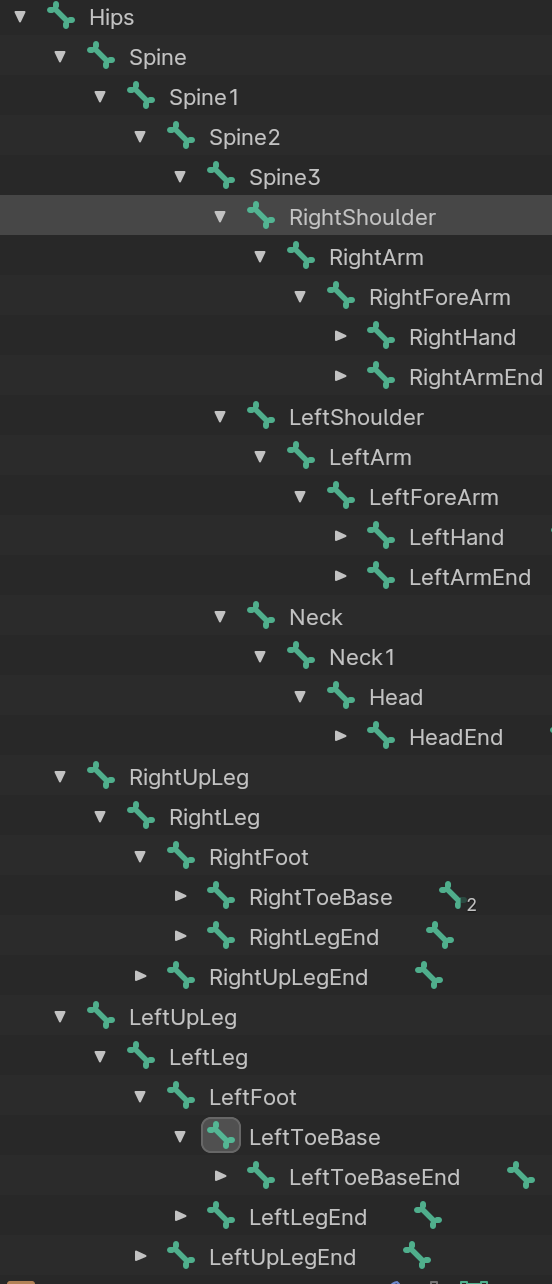
\includegraphics[height=10.5cm]{figures/Bone}
	\caption{Character skeleton}
	\label{fig:Bone}
\end{figure}

\subsection{Structure of a BVH File}
\label{appendix:BVHStructure}

A BVH (Biovision Hierarchy) file is a data format that contains information about the skeleton structure and motion data of bones in a skeletal system. A BVH file consists of two main parts: the skeleton hierarchy declaration and the bone motion data.

\begin{itemize}
	\item \textbf{HIERARCHY}:
	
	\begin{itemize}
		\item Defines the components and names of the skeleton joints, as well as the initial positions of the joints in the T-pose (motion capture actors extend their arms horizontally to form a "T").
		\item Defines the parent-child relationships from the root node to the leaf nodes of the skeleton, typically with the root node being the spine ($\texttt{Spine}$).
		\item Specifies the data to be recorded such as position or rotation angles along $X, Y, Z$ axes of each joint over time.
	\end{itemize}
	
	\item \textbf{MOTION}: A sequence of movements frame by frame, where each frame contains bone movement data as defined in the HIERARCHY section (e.g., rotation angles or positions).
\end{itemize}

\begin{figure}[htbp]
	\centering
	\begin{subfigure}{0.49\linewidth}
		\centering
		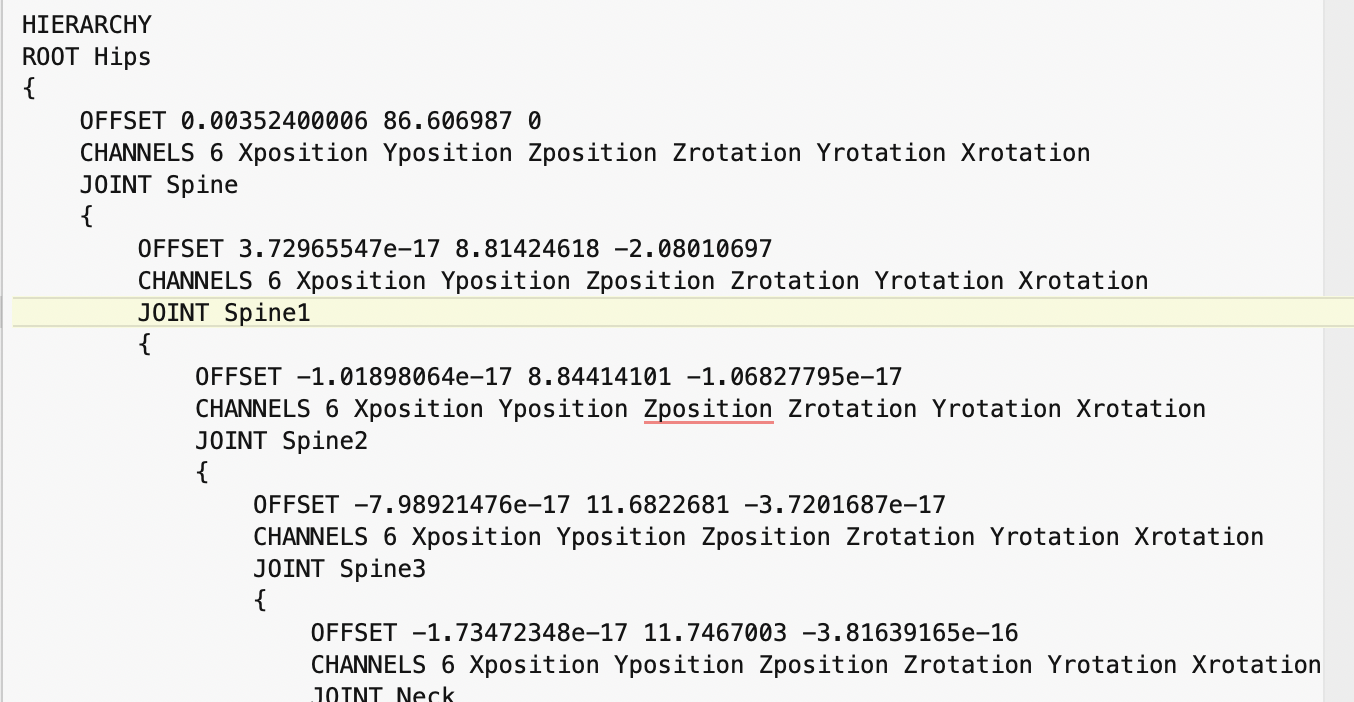
\includegraphics[width=\linewidth]{figures/BVH1}
		\caption{HIERARCHY in BVH file}
		\label{fig:BVH1}
	\end{subfigure}
	\hfill
	\begin{subfigure}{0.49\linewidth}
		\centering
		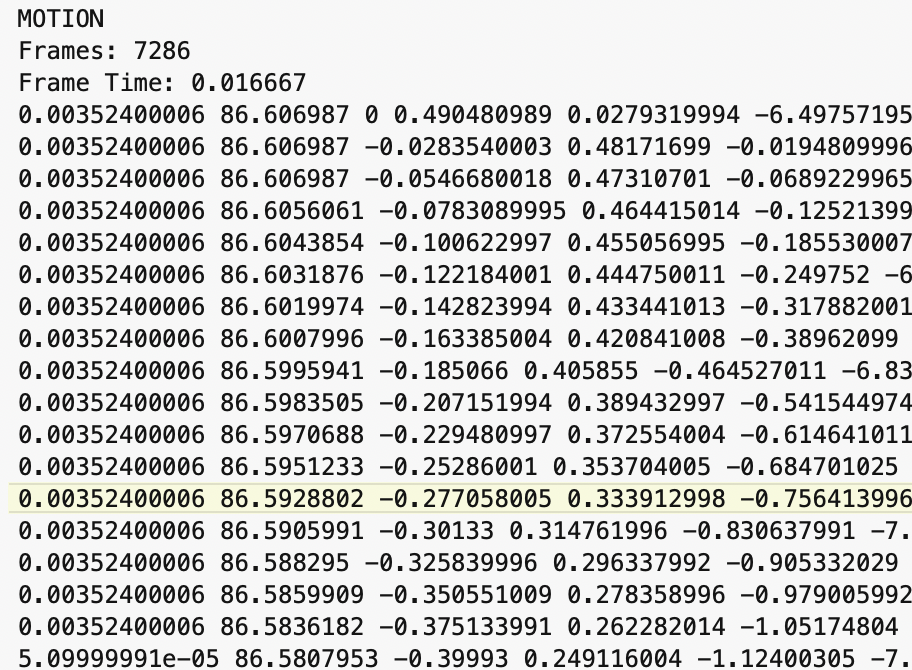
\includegraphics[width=\linewidth]{figures/BVH2}
		\caption{MOTION in BVH file}
		\label{fig:BVH2}
	\end{subfigure}
\end{figure}

$\mathbf{rotation}_i^{\operatorname{local}} = \{ \alpha ,\beta , \gamma \}$ represents the rotation angles around the $Z$, $Y$, and $X$ axes, respectively. The combined rotation in Euler space is:

\begin{equation}
	R = R_Z(\alpha) R_Y(\beta) R_X(\gamma)
\end{equation}

Where:

1. \textbf{Rotation matrix around axis \(Z\)}:

\[
R_Z(\alpha) = 
\begin{bmatrix}
	\cos(\alpha) & -\sin(\alpha) & 0 \\
	\sin(\alpha) & \cos(\alpha) & 0 \\
	0 & 0 & 1
\end{bmatrix}
\]

2. \textbf{Rotation matrix around axis \(Y\)}:

\[
R_Y(\beta) = 
\begin{bmatrix}
	\cos(\beta) & 0 & \sin(\beta) \\
	0 & 1 & 0 \\
	-\sin(\beta) & 0 & \cos(\beta)
\end{bmatrix}
\]

3. \textbf{Rotation matrix around axis \(X\)}:

\[
R_X(\gamma) = 
\begin{bmatrix}
	1 & 0 & 0 \\
	0 & \cos(\gamma) & -\sin(\gamma) \\
	0 & \sin(\gamma) & \cos(\gamma)
\end{bmatrix}
\]

To compute the motion coordinates of a character, the following operation is applied:

\begin{equation}
	\mathbf{position}_{\text{global}} = R \cdot \mathbf{position}_{\text{local}} + \mathbf{t}
\end{equation}


\subsection{Conversion from Euler Angles to Quaternions}
\label{appendix:BVHQuaternion}

To avoid Gimbal lock, Euler angle data must be converted into quaternion representation. Each bone's rotation from Euler angles in the ZYX order is represented as a quaternion $q = (q_w, q_x, q_y, q_z)$, with components calculated as follows:

First, compute the $\cos$ and $\sin$ values of half the rotation angles for each axis:

\begin{itemize}
	\item $c_{\alpha} = \cos\left(\frac{\alpha}{2}\right), \quad s_{\alpha} = \sin\left(\frac{\alpha}{2}\right)$
	\item $c_{\beta} = \cos\left(\frac{\beta}{2}\right), \quad s_{\beta} = \sin\left(\frac{\beta}{2}\right)$
	\item $c_{\gamma} = \cos\left(\frac{\gamma}{2}\right), \quad s_{\gamma} = \sin\left(\frac{\gamma}{2}\right)$
\end{itemize}

Based on the values above, the quaternion components are computed as:

\begin{itemize}
	\item $q_w = c_{\alpha} c_{\beta} c_{\gamma} + s_{\alpha} s_{\beta} s_{\gamma}$
	\item $q_x = c_{\alpha} c_{\beta} s_{\gamma} - s_{\alpha} s_{\beta} c_{\gamma}$
	\item $q_y = c_{\alpha} s_{\beta} c_{\gamma} + s_{\alpha} c_{\beta} s_{\gamma}$
	\item $q_z = s_{\alpha} c_{\beta} c_{\gamma} - c_{\alpha} s_{\beta} s_{\gamma}$
\end{itemize}

With the computed quaternion $q$, the global position of the bone $\mathbf{p}_{\text{global}}$ is determined by rotating the local position $\mathbf{p}_{\text{local}}$ using the formula:

\begin{equation}
	\mathbf{p}_{\text{global}} = q \cdot \mathbf{p}_{\text{local}} \cdot q^{-1} + \mathbf{t}
\end{equation}

where $\mathbf{t}$ is the origin position of the bone in global space.
